\chapter{Introduction to Oscillator Circuits}
\label{chapOscillators}

In Chapter~\ref{chapCapacitorTimer}, we learned how to use RC (resistor-capacitor) circuits to create timers.  
In this chapter, we are going to use our concept of timing circuits to move from one-time timer circuits to \emph{oscillating} circuits.

\section{Oscillation Basics}

So far, most of the circuits we have made have been fairly directional.  
You do an action (i.e., press a button) and then something happens, but then the circuit just maintains a steady-state after that.
In Chapter~\ref{chapCapacitorTimer}, we at least added a delay---allowing the circuit to do something \emph{later}.

However, if you want actions to continue on into the future, you need to not only have delays, you need to have \emph{oscillations}.
\glossterm{Oscillation} means to go back and forth.
An oscillating circuit is one that goes back and forth continually between two states---usually zero voltage and some positive voltage.
Imagine blinking lights at Christmas.
These lights go from a state of zero voltage (off) to a state of positive voltage (on). 
And they go back and forth between these states over and over again as long as there is power in the circuit.
These are oscillating circuits.

An oscillator is usually described by either its \glossterm{period} or its \glossterm{frequency}.
The period of an oscillator is how many seconds it takes to go through one complete cycle.  
So, if I had lights that blinked on for one second and then off for two seconds (and continued repeating in that fashion), the period would be three seconds.

The frequency of an oscillation is the number of times that the system cycles every second, which is merely the reciprocal of the period (i.e., one divided by the period).
So, in the example given, since the period was 3 seconds, the frequency is $\frac{1}{3}$ cycles per second.
The unit ``cycles per second'' also has a special name---\glossterm{hertz} (often abbreviated as hz).
Therefore, we would say that our blinking lights blinked at a frequency of $\frac{1}{3}\myhz$.

\begin{exampleprob}
Let's say that we have an oscillator that turns a light on for four seconds and then turns off for four seconds, and repeats this continually.
What is the period and frequency of this oscillator?

The period is merely the total time it takes to go through one complete cycle.
Therefore:

\begin{align*}
\textrm{period} &= 4\mysec + 4\mysec \\
  &= 8\mysec
\end{align*}

So, what is the frequency of this oscillator?  Simple, just take the reciprocal of the period.  That makes the frequency $\frac{1}{8}\myhz$.
\end{exampleprob} 

\begin{exampleprob}
On a piano, the Middle-C key plays a sound with a frequency of $261.6\myhz$.
What is the period of this sound?

Since the frequency is the reciprocal of the period, it works the other way around as well---period is the reciprocal of the frequency.
Therefore, the period is simply $\frac{1}{261.6}$ seconds.
Or, as a decimal, this is $0.00382$ seconds.
\end{exampleprob}

There are many other factors that are important to various kinds of oscillations, such as the speed of transition between states, what percentage of time each state is achieved, etc.
However, the period/frequency is a good way to summarize the behavior of an oscillator into a single number.

\section{The Importance of Oscillating Circuits}

Oscillating circuits are important in electronics for a number of reasons.
First, obviously, is blinky lights.  
Who goes into electronics without being enamored by blinking lights?
But, more importantly, the following are all applications of oscillators in circuits:
\begin{description}
\item[Sound production] Sounds and tones are made by moving a speaker back-and-forth, which is moved back and forth by electricity oscillating between different voltages.
\item[Time clocks] Every clock on earth operates by an oscillator.  The clock simply counts the number of oscillations that have occurred to know whether or not to advance another minute.
\item[Hardware coordination clocks] In computers and other advanced hardware, system events are coordinated based on signals from an oscillating circuit.  When the clock changes state from off to on, then the circuit does the next step in the process.  The clock keeps the different circuits from interfering with each other.
\item[Radio transmissions] Oscillators are used in radios in order to encode signals onto ``carrier waves,'' which are just oscillating signals run at a specific frequency.
\item[Servo Motors] A servo is a motor which moves an arm to a specific angle (i.e., think of a car's steering).  Servos are usually operated by frequencies, where each frequency specifies a different angle to move.
\end{description}

Let's look in more depth about sound is produced by oscillation.
You hear sound through your eardrum, which communicates vibrations it detects to your brain which you interpret as sound.
Therefore, any sound that you hear is merely the vibrations of your eardrum.
In other words, your eardrum \emph{oscillates} back and forth, which you interpret as sound.

What makes your eardrum move back and forth?
The answer---oscillations in the air.
What makes those oscillations happen?
Oscillations in the sound speaker.
When the speaker moves back and forth, it moves the air which produces sound that you hear.

But what moves the speaker back and forth?
Oscillations in the voltage and current supplied to the speaker.
The speaker has a magnet attached to it which responds to changes in voltage in the wire.
As the voltage in the wire increases, it moves the speaker in one direction.
As the voltage decreases, the speaker moves in the other direction.
Thus, the oscillations in voltage eventually wind up as sound for your ears.

\section{Building an Oscillator}

Let's think for a moment of what it would take to build an oscillator.
On oscillator has (at least) two different states---on and off.\footnote{You can build an oscillator with more than two states, but we won't be concerned with those circuits in this book, though the setup is similar.}
Then, you have a time period between changing from each state to the other.

What sort of circuit have we looked at that provides a time period?

As we saw in Chapter~\ref{chapCapacitorTimer}, RC (resistor-capacitor) circuits can provide us with time delays.
We can then use these time delays as the time periods between the states of the oscillation.
What we need is a circuit that will give out a state (we'll called it S1) for a time period (we'll call it T1) and then move to another state (we'll call it S2) and stay there for another time period (we'll call it T2). 
After T2 is finished, the circuit moves back to state S1 and begins again.

Now, it is possible that we might be able to build such a circuit using multiple RC timers with multiple comparators.
It is doable, but it is harder than it sounds.
Thankfully, there is an integrated circuit that is built for making such timers---the NE555, often referred to as just a ``555 timer'' or just a ``555.''
The NE555 is a very flexible component, and engineers are constantly finding new ways to make use of it.
However, we will just focus on using it as a basic oscillator.

\simplegraphicsfigure{The 555 Pinout Diagram}{555Pinout}{0.08}

It is easiest to describe how a 555 works if we start out by showing a simple circuit with it.
The circuit in Figure~\ref{figSimple555Oscillator} blinks an LED on and off.

\simplepdffigure{A Schematic of a Simple 555 Oscillation Circuit}{Simple555Oscillator}{0.5}

The order of the pins on the actual 555 chip is a little confusing.
In order to make it easier, I have simply put tags for each pin, so you can see where they each belong \emph{functionally}.

First, let's look at the pins on the left-hand side that are directly connected to the power rails.
Pin~1 ($Ground$) and Pin~8 ($VCC$) are easy enough---they are connected to ground and positive voltage, respectively.
Pin~4 ($\overline{Reset}$) gets connected to the voltage source, too.
That is a reset pin which is activated if the pin receives a \emph{low} voltage signal.
Pins that are activated by low-voltage signals are often shown with a line over them.\footnote{Since most pins are activated by a higher voltage, pins that are activated with a lower voltage get the special treatment.}
In our case, we never want to reset the chip, so we will just tie the reset pin to positive voltage which will prevent any accidental resets from changes in voltages in the air.

Now, on the right-hand side at the top, you can see the LED connected to Pin~3 ($Output$).
Pin~3 is simply the output pin.
It is an active output, meaning that it will supply current to the output on its own.  
We don't need a pull-up resistor like we did for the LM393.
Instead, we just need a current-limiting resistor for the LED.
The regular NE555 output yields a voltage that is about $1.7\myvolt$ less than the supply voltage, and sources up to $200\mymamp$ before it breaks.

Note that there are other, low-power versions of the 555 timer that have other output characteristics.
For instance, the LMC555 has an output voltage that is equal to the input voltage, but can only source about $100\mymamp$.
For our purposes, either one would work, as we are not doing anything precise with our output.
However, any calculations we do will assume a typical NE555 component.

On the bottom right Pin~5 ($Control$) is connected through a $10\myuf$ capacitor to ground.
This is just a standard part of using the chip. 
You can't effectively include capacitors in integrated circuits, so many chips specify certain capacitors be attached to certain pins.
The NE555 uses a $10\myuf$ capacitor on Pin~5 to provide voltage stability.
In Chapter~\ref{chapCapacitors}, we learned that capacitors act essentially like little batteries.
This capacitor is doing just that.
It is providing a short-term supply of charge in case there is a sudden change in current needs within the chip.
For instance, when the output goes active, there may be a sudden need for charge.
This capacitor supplies a quickly available reservoir of charge available to the chip so that sudden changes in current needs will not affect other chip properties.\footnote{For most of our uses of the NE555, you can actually leave Pin~5 unconnected---our usage of the chip are not so precise or power-hungry as to be affected in this way.  
Nonetheless, I show it connected so that you can see how it is \emph{supposed} to be connected.}

Down the middle of the schematic is where all of the action happens.
This is what controls the oscillation.
It is essentially an RC circuit with (a) an extra resistor, and (b) a few tie-ins to the chip.
As we will see shortly, the capacitor will alternately charge and discharge.
The capacitor itself is attached to two voltage sensors on the chip.
The first sensor, $\overline{Trigger}$ watches the voltage on the capacitor, and activates if the voltage falls below $\frac{1}{3}$ of the supply voltage (the line over the name of the pin indicates that it activates on a low value).
The second sensor, $Threshold$, watches the voltage, and will activate if the voltage goes above $\frac{2}{3}$ of the supply voltage.

So, the oscillator works by moving the capacitor voltage back-and-forth between $\frac{1}{3}$ and $\frac{2}{3}$ of the supply voltage.
It is fairly obvious to see how the capacitor charges---it is a basic RC circuit using both of the resistors R1 and R2.
So how does the capacitor discharge?
The capacitor discharges through the action of the $Discharge$ pin, Pin~7.
When the 555 starts up, Pin~7 essentially acts as if it were not connected to anything, so you can basically ignore it.
When the capacitor goes over the $\frac{2}{3}$ supply voltage and triggers the $Threshold$ pin, the 555 will then connect Pin~7 to ground.

Think about what will happen if Pin~7 is connected to ground.
Will the capacitor charge?
No, the current coming in through R1 will immediately go to ground because it is the easiest path.
If the capacitor is charged up, is it above or below ground?
It is obviously above ground.
Therefore, current will flow \emph{out of} the capacitor, through R2, and to ground.
Thus, the capacitor discharges, but at a \emph{different} rate than it charged.
The RC circuit for the charging of the capacitor used both R1 and R2 for the resistance.
However, the discharge of the capacitor only uses R2.
Therefore, the discharge from $\frac{2}{3}$ voltage down to $\frac{1}{3}$ voltage will be faster than the charge up.

Once the capacitor discharges down to $\frac{1}{3}$ of supply voltage, Pin~2 ($\overline{Trigger}$) will detect this event and turn Pin~7 off so that the capacitor can recharge again.
Therefore, the capacitor will be continually charging and discharging through $\frac{1}{3}$ to $\frac{2}{3}$ of supply voltage, as the 555 turns Pin~7 (connected to ground) on and off.
This is also why having two resistors is so important.
If we didn't have R1, when Pin~7 connected to ground it would make a short circuit between the supply voltage and ground.

You may be wondering why there are two detectors connected to the capacitor and not just one.
The reason for this is that having two different detectors allows for a \emph{lot} of flexibility in how the 555 is wired.
As mentioned earlier, there are a huge number of ways the 555 has been used, and some uses tie $\overline{Trigger}$ and $Threshold$ to different parts of the circuit.
For our purposes, both of these will always be used together.

So, how does this charging and discharging of the capacitor affect the output?
Quite simply, when the capacitor is \emph{charging}, the output is \emph{on}.
When the capacitor is \emph{discharging}, the output is \emph{off}.
Note that when we first turn on the 555, the output will be on for a little bit longer than for the rest of the time.
This is simply because when the circuit first starts up it is charging all the way from $0\myvolt$ instead of from $\frac{1}{3}$ of supply voltage.

\simplegraphicsfigure{The 555 Oscillator Circuit on a Breadboard}{Simple555OscillatorBreadboard}{1}

You can see the completed 555 circuit on a breadboard in Figure~\ref{figSimple555OscillatorBreadboard}.
This should blink the light on for about two thirds of a second and off for about a third of a second.
This gives the total period of about 1 second, and a frequency of about $1\myhz$.
In the next section, we'll see how to use RC time constants to calculate our own timings.

\section{Calculating On and Off Times with the 555}

Remember that the capacitor is charging and discharging through an RC circuit.
Therefore, we can use what we know about RC circuits to determine how long the circuit will be high and low.

When the capacitor is \emph{charging}, the capacitor is charging through \emph{both} R1 and R2.
In this situation, what is the RC time constant?
Well, since the resistance is a series resistance, we can simply add them together:

\begin{align*}
R_T &= R_1 + R_2 \\
    &= 50,000 + 50,000 \\
    &= 100,000
\end{align*}

So the resistance is $100,000\myohm$ and we are using a $10\myuf$ capacitor (which is $0.00001\myf$).
Therefore (based on Chapter~\ref{chapCapacitorTimer}), the RC time constant is $100,000 \cdot 0.00001 = 1$.
So our RC time constant is 1 second.
However, we are charging/discharging the capacitor in a strange way.
We are not starting from zero (except for the first time)---instead we are usually starting from $\frac{1}{3}$ of supply voltage.

Go back to Chapter~\ref{chapCapacitorTimer} and look at Figure~\ref{figTimeConstants}.
While we don't have a time constant for \emph{exactly} $\frac{1}{3}$ of supply voltage, we do have one for $39.3\%$, which is pretty close.
So, in the table, that occurs as $0.5$ time constants.
In this case, that is our \emph{starting} value.
Our ending value is when the capacitor is $\frac{2}{3}$ charged.
That is very close to $63.2\%$, which is at one time constant.
Therefore, the \emph{difference} between the point where we are $\frac{1}{3}$ charged and $\frac{2}{3}$ charged is $1 - 0.5 = 0.5$ time constants.

Since we were using approximate values from the table, this is only an approximation.
The circuit actually use a little longer period than that.
It turns out that to go from $\frac{1}{3}$ supply voltage to $\frac{2}{3}$ supply voltage actually takes 0.693 time constants.
This is an important number to remember when when using the NE555, as it will be used in all of your time calculuations.
Since our time constant is 1 second, that makes the calculation really easy: $1\cdot 0.693 = 0.693\mysec$.

Now, for discharge, remember that the point that it is discharging to is Pin~7.
This is \emph{between} R1 and R2.
That means that it is \emph{only} using R2 to discharge, so the RC time constant will be based only on R2 and the capacitor.
So, the RC time constant is $50,000 \cdot 0.00001 = 0.5\mysec$.
Since the charge/discharge time between $\frac{1}{3}$ and $\frac{2}{3}$ is $0.693$ time constants, the resulting time to discharge from from $\frac{2}{3}$ down to $\frac{1}{3}$ is $0.693 \cdot 0.5 = 0.347\mysec$.

The total period will be the total time for one cycle
This will be our charge time ($0.693\mysec$) plus the discharge time ($0.347\mysec$) which will give us a total of $1.04\mysec$.

The value $0.693$ looks like a strange number, but that will \emph{always} be the value used for th number of time constants for charging/discharging between $\frac{1}{3}$ and $\frac{2}{3}$ of supply voltage.
If you are going to use the 555 timer, it is best to just memorize it.

Also note that since the charging goes through \emph{both} resistors while the discharge only goes through \emph{one} resistor, the charge time (with the output on) will \emph{always} be longer than the discharge time (with the output off).

\begin{exampleprob}
Let's say we have the basic oscillator circuit shown in Figure~\ref{figSimple555Oscillator}, but with a $2,000\myohm$ resistor for R1, a $6,000\myohm$ resistor for R2, and a $10\myuf$ capacitor for C1.  What will be the charge time, the discharge time, the period, and the frequency for our oscillator?

To find this out, it is easiest to first calculate the charge and discharge times separately, and then use those to find period and frequency.
The charge time will be calculated based on \emph{both} resistors in our RC circuit.
So the resistance will be $2,000\myohm + 6,000\myohm = 8,000\myohm$.
The capacitance is $10\myuf = 0.00001\myf$.
This means that the RC time constant will be $8,000\myohm \cdot 0.00001\myf = 0.08\mysec$.

The number of time constants it takes to charge from $\frac{1}{3}$ to $\frac{2}{3}$ is 0.693.
This means that the charge time will be $0.08 * 0.693 = 0.0554\mysec$.

The discharge happens only through R2.
This means that the RC time constant will be $6,000\myohm \cdot 0.00001\myf = 0.06\mysec$.
Since we will use 0.693 time constants, the total time it takes to discharge from $\frac{2}{3}$ down to $\frac{1}{3}$ is $0.693 * 0.06 = 0.0416\mysec$.

Now that we have the charging and discharging times, we find the period by merely adding them together.
This means the period is $0.0554 + 0.0416 = 0.097\mysec$.

The frequency is merely the reciprocal of this number, or $\frac{1}{0.097}$, which gives us $10.3\myhz$.
\end{exampleprob}

\begin{exampleprob}
Now let's say that we want to build an oscillator for which the LED stays on for 3 seconds and then goes off for 2 seconds.
Assuming we keep our $10\myuf$ capacitor, what values should we use for each resistor?

To do this, we need to solve for R2 first, since it is much easier.
The discharge will be 2 seconds, which will be the same as $0.693 \cdot \textrm{time constant}$.
Therefore, we can write this as an equation:

\begin{align*}
2\mysec &= R\cdot C\cdot 0.693 \\
2\mysec &= R\cdot 0.00001 \cdot 0.69 \\
2\mysec &= R\cdot 0.0000069 \\
\frac{2\mysec}{0.0000069} &= R \\
289,855\myohm &\approx R
\end{align*}

So, the resistor, R2, needs to be $289,555\myohm$.

The time to charge the capacitor, however, needs to be $3\mysec$.
This means the resistance (which will be \emph{both} R1 and R1) will need to be calculated for this as well.
Therefore, we will use a similar equation:

\begin{align*}
3\mysec &= R\cdot C\cdot 0.693 \\
3\mysec &= R\cdot 0.00001\myf \cdot 0.693 \\
3\mysec &= R\cdot 0.00000693 \\
\frac{3\mysec}{0.00000693} &= R \\
434,783\myohm &= R
\end{align*}

So the resistance for charging the capacitor needs to be $434,783\myohm$.
However, this is the \emph{combined} resistance for R1 and R2.
Thankfully, though, we already know what we want for R2---$289,855\myohm$.
Therefore, we can put these into an equation and solve for R1:

\begin{align*}
R_1 + R_2 &= 434,783\myohm \\
R_1 + 289,855\myohm &= 434,783\myohm \\
R_1 &= 434,783\myohm - 289,855\myohm \\
R_1 &= 144,928\myohm
\end{align*}

So now we know our values for R1 and R2---$144,928\myohm$ and $289,855\myohm$.
Depending on our application, we would probably simply choose resistors that were close to that amount (like $150\mykohm$ and $300\mykohm$) rather than trying to find a combination of resistors that hit that precise resistance.
But, for solving equations, it is best to use exact values.
\end{exampleprob}

%% FIXME - should probably do a chapter on IC block diagrams and show how to build an NE555 from scratch
%% FIXME - should I show other configurations of the 555?

\section{Choosing the Capacitor}

Ultimately, there are no hard-and-fast rules for choosing capacitors.  
As long as the RC time constant yields the right value, then you can compensate for pretty much any size capacitor with the right size of resistor.
However, sometimes just having a little guidance helps people get started, and there are a few situations that you need to watch out for.

First of all, the size of capacitor will affect the size of resistor you need for a given time constant.
If all you have are smaller-sized resistors, then you should probably use a larger capacitor to compensate.

However, using a smaller capacitor with larger resistors gives a very large advantage in the amount of wasted current.
If you are using smaller resistors, then Ohm's law indicates that we will have larger currents for a given voltage.  
Since $V = I\cdot R$, if you lower the $R$ you will increase the $I$.
So, having a higher resistance means that your RC circuit will use much less current.

Remember that we aren't actually \emph{using} the current to \emph{do} anything except keep time. 
The current in our RC circuit is not used to power the LED (the 555 does that through the power source), it isn't used for anything else, it is just used to keep time.
Therefore, pretty much all current used by the RC circuits is wasted.
We have to use it, but any smaller currents we can get away with, we should!

This gets even more pronounced when the capacitor is discharging.
When Pin~7 ($DISCHARGE$) switches to ground, not only does it discharge the capacitor, but it also creates a useless waste of current going from the voltage source through R1.
In our oscillator configuration, you can't get rid of this, but having larger resistors will reduce the amount waste.

So, in short, if you have higher-valued resistors to compensate, your circuit will waste much less current by using smaller capacitors.

\reviewsection

In this chapter, we learned:

\begin{enumerate}
\item Because this material is based so heavily on RC circuits, you may want to review the material in Chapter~\ref{chapCapacitorTimer}.
\item When something oscillates it moves back and forth between a set of values.
\item In electronics, oscillators usually refer to circuits whose output voltages go back and forth between two different values.
\item Oscillations are usually described by their period or frequency.
\item The period of an oscillation is the time that it takes to go through one entire cycle (usually in seconds).
\item The frequency of an oscillation is the number of times that an oscillation occurs per second, which is simply the reciprocal of the period (i.e., $\frac{1}{\textrm{period}}$), with a unit of hertz (cycles per second).
\item Oscillating circuits are used in a number of circuit applications, including sound production, time keeping, coordinating activities, radio transmissions, and motor control.
\item Oscillating circuits are often built with RC time circuits which control the time periods of the oscillations.
\item The NE555 (often referred to as a 555 timer or just the 555) is an integrated circuit which allows for several timing applications including making oscillating circuits.
\item The NE555, when setup as an oscillator, is controlled by two resistors and a capacitor.
\item The NE555 can be setup to monitor the charge of the capacitor.  It has two pins for monitoring the voltage, $\overline{Trigger}$ (which checks for the capacitor to drop below $\frac{1}{3}$ supply voltage, and $Threshold$ (which checks to see when the capacitor is charged above $\frac{2}{3}$ of supply voltage.
\item The NE555 cycles between charging and discharging the capacitor from $\frac{1}{3}$ of supply voltage to $\frac{2}{3}$ of supply voltage and back (using $\overline{Trigger}$ and $Threshold$ to check the voltage level).
\item The $Discharge$ pin of the NE555 acts like it is disconnected when the capacitor is charging, and is connected to ground to allow for a path for the capacitor to discharge.
\item The $Output$ pin of the NE555 is turned on (higher voltage level) while the capacitor is charging, and off (low voltage level) when the capacitor is discharging.  The NE555 output operates at about $1.7\myvolt$ less than the source voltage when on, and can source a maximum of $200\mymamp$ to the output circuit.
\item The $\overline{Reset}$ pin can be given a low voltage to reset the whole device.  If it is unused, it should just be tied to a positive voltage line.
\item The $Control$ pin is attached to a capacitor in order to regulate and stabilize the circuit operation.
\item The RC circuit takes $0.693$ time constants to charge from $\frac{1}{3}$ voltage to $\frac{2}{3}$ voltage or to discharge the other way.  Therefore, once you have the RC time constant, multiply by $0.693$ to find the actual time it will take.
\item The RC circuit utilizes \emph{both} resistors when charging, but only \emph{one} resistor when discharging.  This means that charging and discharging each have their own RC time constants.
\item Because the charge circuit uses two resistors while the discharge circuit only uses one, the charging portion of the oscillation period will always be at least a little longer than the discharging portion.
\item The period of the oscillation is the combination of both the charge time and the discharge time.
\item When calculating resistors for an RC time circuit, it is best to calculate the discharge resistance first, since it only uses one resistor (R2).  Then you can calculate the combined resistance for the charge circuit, which allows you to deduce what the R1 resistor should be.
\item When choosing components for a given RC time constant, you can choose a variety of combinations of capacitor/resistor values for the same result.  Choosing a smaller capacitor and a larger resistor will save power in the circuit.
\item An equation for determining the frequency of a 555 oscillator circuit can be found in Appendix~\ref{apOscillatorFreq}.
\end{enumerate}

\applysection


\begin{enumerate}
\item 
\question{Take a look at the circuit in Figure~\ref{figSimple555Oscillator} (this will be used as the basis for the problems in this section).   Copy this circuit to a piece of paper.  Draw a line in one color showing how the current flows in the main circuit as it charges the capacitor.  With a different color, draw a line showing how current flows as the capacitor discharges.  Use arrows to indicate current direction.  You can ignore the ``Output'' and ``Control'' sections of the circuit for this problem.}
\solution{The lines should be drawn as follows:\newline
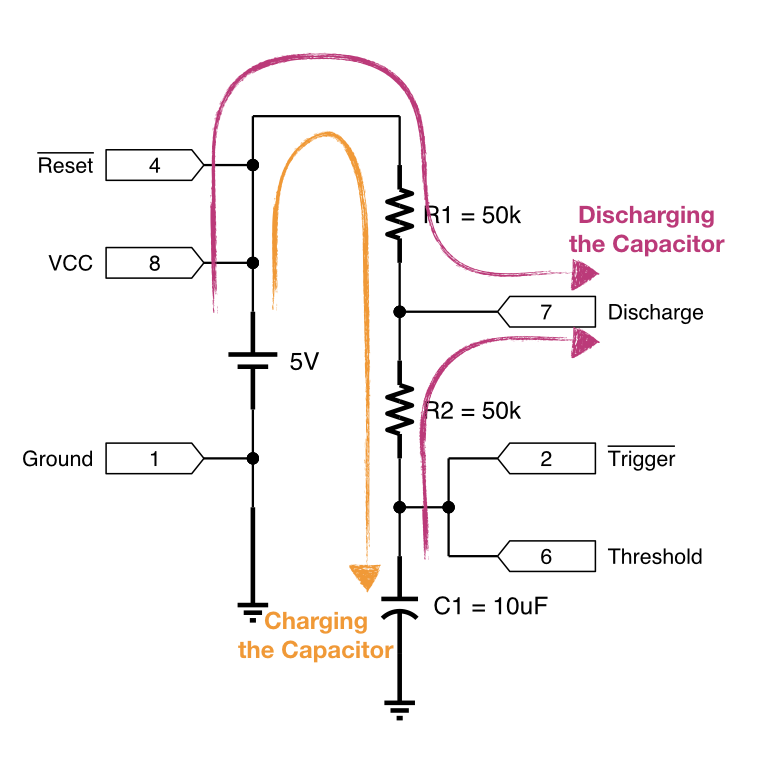
\includegraphics[width=0.8\columnwidth]{ExOscillatorChargeDischarge.png}
}
\explanation{
During the charging phase, current flows from the positive all the way into the capacitor.
This is shown with the line that is on the interior of the circuit.
During the discharge phase, Pin~7 goes low, and therefore current flows into Pin~7 from \emph{both}
the power supply \emph{and} from the capacitor.
}
\item 
\question{Why is R1 important?  What would happen if we just replaced it with a wire?}
\solution{During the discharge phase, R1 acts as a current-limiting resistor.  It would create a short-circuit from power to ground if it was just a wire.}
\explanation{Remember, there is no intelligence in a circuit.
The power supply only knows how to supply power.
Therefore, during the discharge phase, the power supply \emph{will continue to supply power just as before}.
When Pin~7 goes to zero volts, not only does the charge from the capacitor start to flow in that direction, but also the power from the supply.
If there is no resistor here, then it becomes a short-circuit from supply to ground.
Additionally, since this power is entirely wasted, R1 also limits the amount of waste that occurs during the discharge phase.
}
\item 
\question{Why are there two different pins on the NE555 connected to the capacitor?  What type of circuit (that we have discussed in this book) do you think they are connected to inside the chip?}
\solution{One compares for voltage \emph{above} a certain level, and the other compares for voltage \emph{below} a certain level.  Since they are checking for voltage, they are probably voltage comparator circuits.}
\explanation{The NE555, in its standard configuration, allows the capacitor to charge until it is two thirds full, and then discharges it until it is only one third full.
It has to detect for each of these conditions.
Therefore, it has two separate sensing inputs, one for each condition.  
$Threshold$ watches for the high voltage (and switches it from ``charge'' to ``discharge'' when it goes over), and $\overline{Trigger}$ watches for the low voltage (and switches it from ``discharge'' to ``charge'' when it goes under).
Since it is watching voltage levels, it is likely using a voltage comparator in the chip to measure these voltages.
}
\item 
\question{Why is the charging time of the NE555 always at least a little longer than the discharging time?}
\solution{The circuit uses both R1 and R2 to charge, but \emph{only} uses R2 to discharge.  Therefore, the resistance for discharging will always be less than the resistance for charging.}
\item 
\question{Why does the NE555 stay in the on state a little longer when the circuit is first turned on?}
\solution{Generally, the NE555 oscillates between filling and discharging the capacitor from one third to two-thirds full.  When first turned on, the capacitor will (presumably) be \emph{fully} discharged, so it will take some amount of time for that first charge cycle to occur, because it is charging from zero instead of from one third full.}
\item 
\question{Let's say that we wanted our circuit to be on for $2\mysec$ and off for $1\mysec$.  Keeping the same capacitor, what values should we use for R1 and R2 to accomplish that?}
\solution{R1 would be $144300.2\myohm$ and R2 would be $144300.1\myohm$.  In terms of standard components, using a $150\mykohm$ resistor for each one would be sufficient.}
\explanation{Since the discharge phase (when the output is off) only uses one resistor (R2) we will beging considering the discharge phase.
The total time is $1\mysec$.
Since we are using a NE555 timer, this time will cover $0.693$ time constants.
The time constant is given by the resistance multiplied by the capacitance.
Since the capacitor is a $10\myuf$ capacitor, the full equation is:
\begin{align*}
R \cdot 0.00001 \cdot 0.693 &= 1 \\
R &= \frac{1}{0.00001 \cdot 0.693} \\
R &\approx 144300.1
\end{align*}
Therefore, R2 will be approximately $144300.1\myohm$.
We now do a similar operation to find R1.  
However, the ``on'' phase of the oscillation will utilize both R1 and R2, and will take two seconds.
Therefore, we can solve for R1 as follows:
\begin{align*}
0.00001 \cdot (144300.1 + R) &\cdot 0.693 = 2 \\
144300.1 + R &= \frac{2}{0.00001 \cdot 0.693} \\
R &= \frac{2}{0.00001 \cdot 0.693} - 144300.1 \\
R &\approx 144300.2 
\end{align*}
So R1 will be approximately $144300.2\myohm$.

Resistors are not actually available in these values.
Therefore, you would likely choose a $150\mykohm$ resistor for each of these.
}
\item 
\question{Let's say that we wanted our circuit to be on for $10\mysec$ and off for $3\mysec$.  Keeping the same capacitor, what values should we use for R1 and R2 to accomplish that?}
\item 
\question{The factory called and said that they were out of the capacitor we wanted for the circuit, and instead only had a $23\myuf$ capacitor that we could use.  Recalculate the previous problem using this new capacitor value.}
\item 
\question{How much current is our output sourcing from the chip?}
\item 
\question{When the chip first turns on (and thus the capacitor is empty and at $0\myvolt$) how much current is the RC circuit using?}
\end{enumerate}

% FIXME - might have a problem where people draw the pinout of the 555
% FIXME - might have a problem where they draw a circuit and then circle different part

